\subsection{Brain Tumor Datenset} \label{chap:Brain-Tumor}
\subsubsection{Hirntumor} \label{chap:Hirntumor}
Hirntumoren sind abnorme Zellwucherungen im Gehirn, die gutartig oder bösartig sein können. Diese Tumoren können entweder direkt im Gehirn entstehen oder als Metastasen von anderen Krebsarten in das Gehirn gelangen. Die Symptome variieren je nach Tumorart, -grösse und -lokalisation und umfassen häufig Kopfschmerzen, Übelkeit, Sehstörungen, Krampfanfälle und kognitive Beeinträchtigungen. Aufgrund ihrer Komplexität und der sensiblen Lage im zentralen Nervensystem stellen Hirntumoren eine erhebliche Herausforderung für die medizinische Diagnostik und Behandlung dar. Sie haben oft weitreichende Auswirkungen auf die Lebensqualität der Betroffenen.

\subsubsection{Datensatz} \label{chap:brain-datensatz}
Der \textbf{Brain Tumor Classification (MRI)-Datensatz} \cite{bhuvaji_brain_2020} umfasst 3.260 bereinigte und augmentierte, T1-gewichtete, kontrastverstärkte MRI-Bilder zur Identifikation und Klassifikation von Hirntumoren.

Die in der Abbildung gezeigten MRI-Bilder illustrieren Beispiele von Gehirnscans, die zur Klassifikation von Hirntumoren verwendet werden. Positive Fälle sind mit der Klasse 1 und negative Fälle mit der Klasse 0 gekennzeichnet. Eine detaillierte Beschreibung der Klassenzusammenfassung findet sich in Kapitel \ref{chap:brain-datapartition}. In den Beispielabbildungen \ref{fig:brain-beispiele-klasse0} und \ref{fig:brain-beispiele-klasse1} ist erkennbar, dass der Datensatz Sagittal-, Frontal- und Transversalebenen des Kopfes enthält.

\begin{figure}[H]
    \centering
    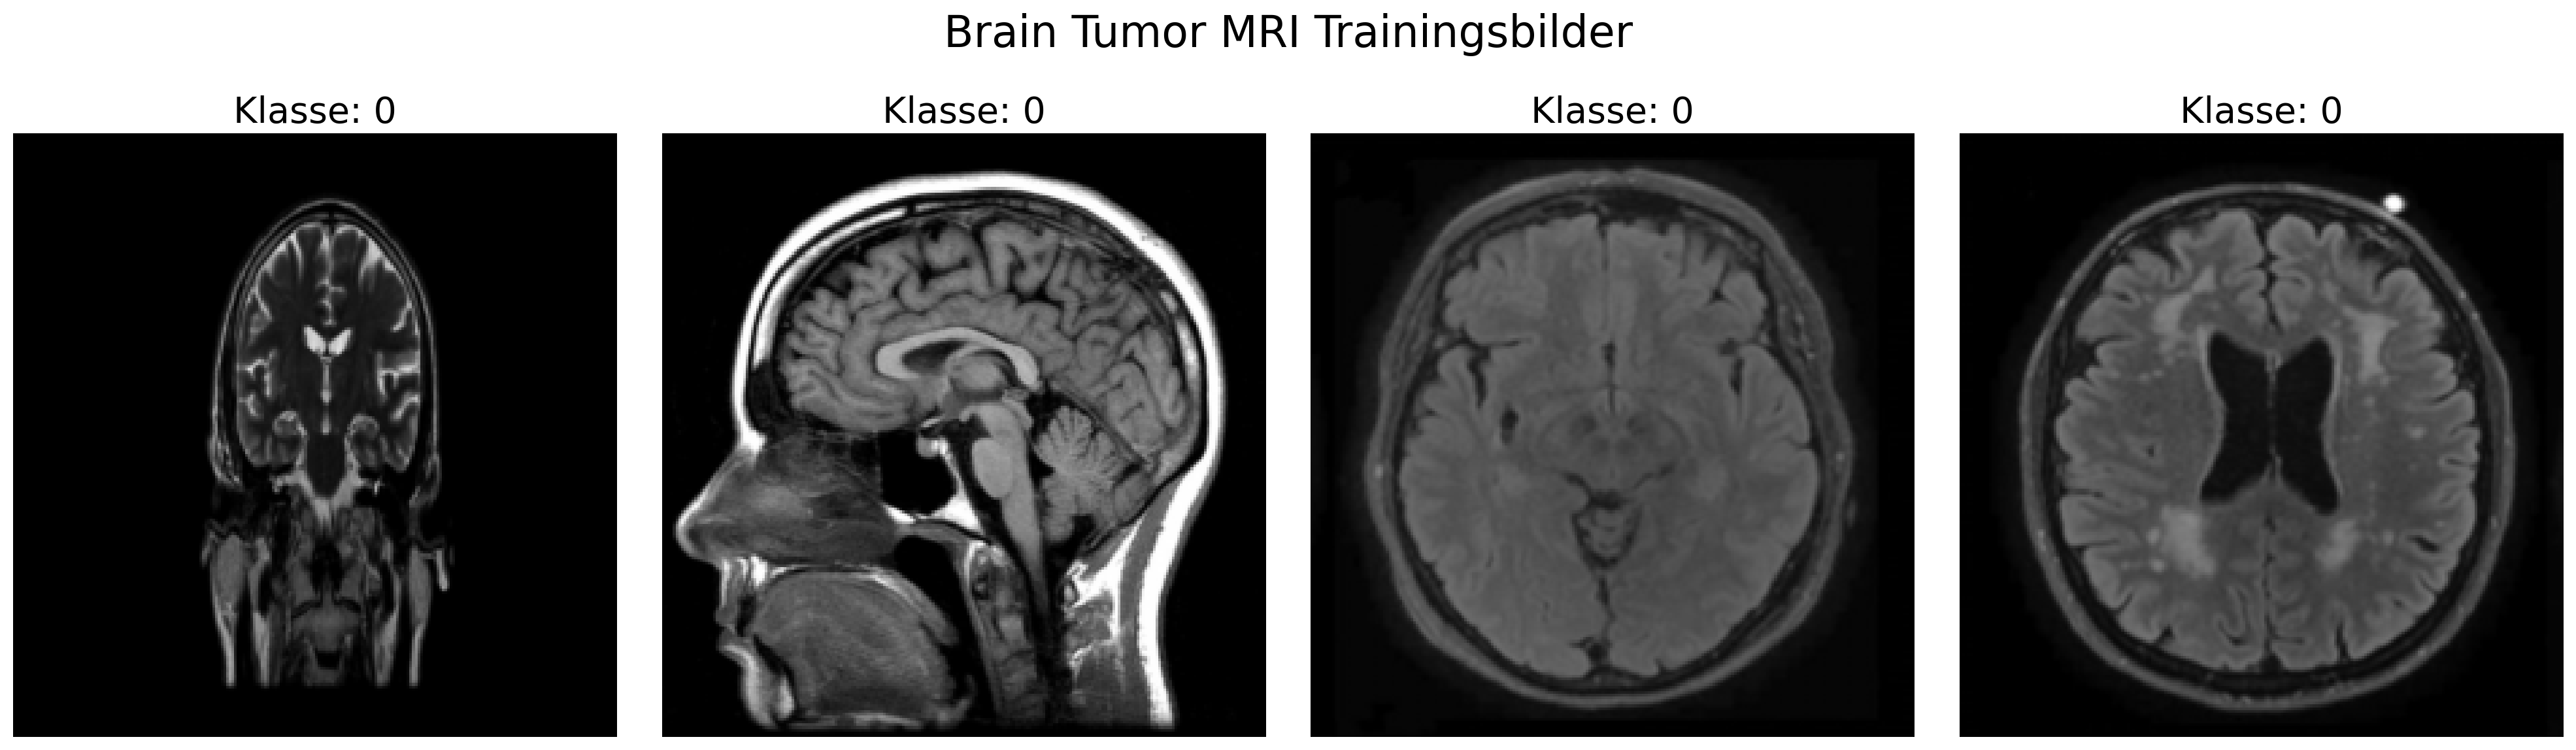
\includegraphics[width=\linewidth]{01-images/03-data/brain-klasse0.png}
    \caption{Beispiele von negativen Hirntumor Patienten vom Brain Tumor Datensatz}
    \label{fig:brain-beispiele-klasse0}
\end{figure}

\begin{figure}[H]
    \centering
    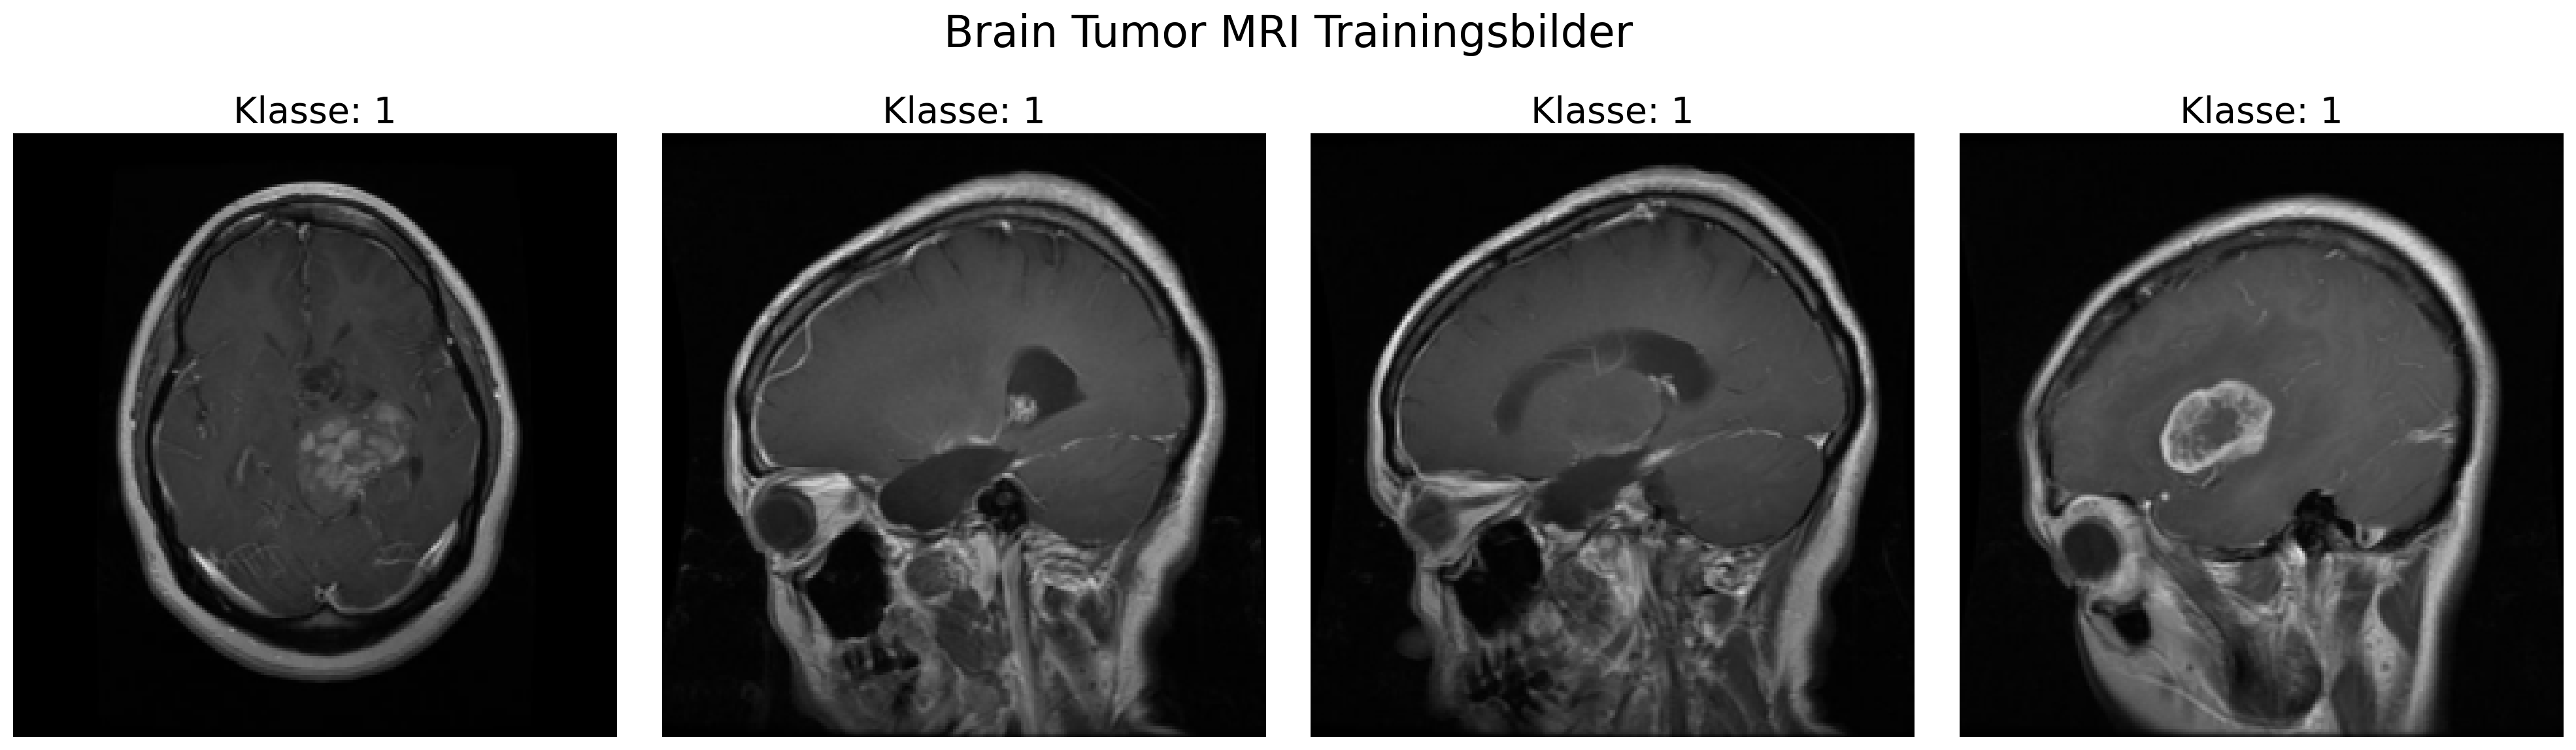
\includegraphics[width=\linewidth]{01-images/03-data/brain-klasse1.png}
    \caption{Beispiele von positiven Hirntumor Patienten vom Brain Tumor Datensatz}
    \label{fig:brain-beispiele-klasse1}
\end{figure}

\subsubsection{Hirntumorarten im Datensatz} \label{chap:brain-hirnarten-datensatz}
Der Datensatz für Hirntumoren umfasst vier Klassen. Drei davon sind positive Fälle, in denen Hirntumoren vorhanden sind, und eine Klasse ist negativ und enthält keine Hirntumoren. Die drei positiven Klassen sind Gliome, maligne Tumoren und Pituary.

\paragraph{Gliome} \label{chap:brain-gliome}
Gliome bilden eine Gruppe von Hirntumoren, die im Glia-Gewebe des Nervensystems entstehen. Sie stellen die häufigsten primären Hirntumoren bei Erwachsenen dar und werden nach ihren Ursprungszellen in Astrozytome, Oligodendrogliome und Ependymome unterteilt. Die Symptome variieren je nach Lage und Grösse des Tumors und umfassen häufig Kopfschmerzen, Anfälle und neurologische Defizite. Die Behandlung erfolgt meist durch eine Kombination aus Operation, Strahlentherapie und Chemotherapie.

\paragraph{Malignent} \label{chap:brain-malignent}
Maligne Tumoren sind bösartige Wucherungen, die unkontrolliert wachsen und in umliegendes Gewebe eindringen können. Sie haben die Fähigkeit, Metastasen zu bilden, das bedeutet, dass sie sich auf andere Teile des Körpers ausbreiten können. Die Behandlung umfasst in der Regel eine Kombination aus Operation, Strahlentherapie und Chemotherapie. Die Prognose hängt von der Art, dem Stadium und der Lage des Tumors ab.

\paragraph{Pituary} \label{chap:brain-pituary}
Pituary, auch als Hypophysenadenome bekannt, sind gutartige Tumoren der Hypophyse, einer kleinen Drüse im Gehirn, die wichtige Hormone produziert. Obwohl sie meist nicht bösartig sind, können sie aufgrund ihrer Lage und Hormonproduktion erhebliche gesundheitliche Probleme verursachen. Zu den Symptomen zählen häufig Kopfschmerzen, Sehstörungen und hormonelle Ungleichgewichte. Die Behandlung erfolgt in der Regel durch eine Operation und, in einigen Fällen, durch medikamentöse Therapie oder Strahlentherapie.

\subsubsection{Datenpartitionierung} \label{chap:brain-datapartition}
Der Datensatz enthält ursprünglich nur ein Trainings- und ein Testset. Da ein Validierungsset fehlt, wird dieses aus dem gegebenen Trainingsset erstellt. Der Datensatz umfasst vier Klassen: drei Tumorklassen und eine Nicht-Tumorklasse. Die Verteilung der Klassen ist in der Tabelle \ref{tab:brain-orginale-klassenverteilung} dargestellt. Es zeigt sich, dass positive Tumorklassen deutlich häufiger vertreten sind als Nicht-Tumore. Da die These auf einer binären Klassifikation basiert, werden die drei Hirntumorklassen Pituitary, Glioma und Meningioma zu einer positiven Gehirntumorklasse zusammengefasst, während die Nicht-Tumorklasse als negative Klasse definiert wird. Dies ergibt die Tabelle \ref{tab:brain-binaere-klassenverteilung}.

\begin{table}[H]
    \centering
    \begin{tabular}{@{}ccccc@{}}
        \toprule
         Partition & \multicolumn{4}{c}{Klassenverteilung}              \\ 
        \cmidrule(l){2-5}
                    & Pituitary & Glioma & Meningioma & kein Tumor      \\ 
        \midrule 
        Train      & 662 & 661 & 658 & 317                              \\
        Validation & 165 & 165 & 164 & 78                               \\
        Test       & 74  & 100 & 115 & 105                              \\ 
        \bottomrule
    \end{tabular}
    \caption{Ursprüngliche Klassenaufteilung von Hirntumoren}
    \label{tab:brain-orginale-klassenverteilung}
\end{table}

Die ursprüngliche Verteilung der Daten umfasste 70,4 \% Trainings- und 29,6 \% Testbilder. Zur vereinfachten Handhabung, wurde aus dem Trainingsdatensatz durch stratifiziertes Sampling ein Trainings- und Validierungsdatensatz erstellt. Dabei wurde darauf geachtet, dass das Validierungsset das gleiche Verhältnis von positiven und negativen Fällen aufweist wie das Trainingsset. Dies wurde gemacht, damit das Format der Partitionen analog wie die vom Covid Datensatz ist. Tabelle \ref{tab:brain-binaere-klassenverteilung} zeigt die Anzahl der Bilder in absoluter und relativer Häufigkeit sowie die Klassenverteilung von positiven und negativen Tumorbildern für jede Datenpartition.

Die ursprüngliche Datenverteilung umfasste 70,4 \% Trainings- und 29,6 \% Testbilder. Für eine vereinfachte Handhabung wurde aus dem Trainingsdatensatz durch stratifiziertes Sampling ein Trainings- und Validierungsdatensatz erstellt. Dabei wurde darauf geachtet, dass das Validierungsset das gleiche Verhältnis von positiven und negativen Fällen wie das Trainingsset aufweist. Dies diente dazu, ein vergleichbares Format wie beim Covid Datensatz zu gewährleisten. Tabelle \ref{tab:brain-binaere-klassenverteilung} zeigt die Anzahl der Bilder in absoluter und relativer Häufigkeit sowie die Klassenverteilung von positiven und negativen Tumorbildern für jede Datenpartition.

\begin{table}[H]
    \centering
    \begin{tabular}{@{}cccccc@{}}
        \toprule
        Partition & \multicolumn{2}{c}{Anzahl Bilder} & \multicolumn{2}{c}{Klassenverteilung} & Positiv-Verhältnis\\ 
        \cmidrule(lr){2-3} \cmidrule(lr){4-5} 
                   & Absolut & Relativ & Positiv & Negativ  \\ 
        \midrule
        Train      & 2298 & 0.704 & 1981 & 317 & 0.862      \\
        Validation & 572  & 0.175 & 494  & 78  & 0.864      \\
        Test       & 394  & 0.121 & 289  & 105 & 0.736      \\ 
        \bottomrule
    \end{tabular}
    \caption{Binäre Klassenverteilung von Hirntumoren}
    \label{tab:brain-binaere-klassenverteilung}
\end{table}

\subsubsection{Datenexploration} \label{chap:brain-eda}
Die Histogramme der Hirntumorklassifikation unterscheiden sich deutlich von denen des COVIDx CXR-4 Datensatzes aus Kapitel \ref{chap:COVID19-eda}. In den Beispielen ist klar ersichtlich, dass die Intensität niedrigerer Pixelwerte sehr hoch ist.

\begin{figure}[H]
    \centering
    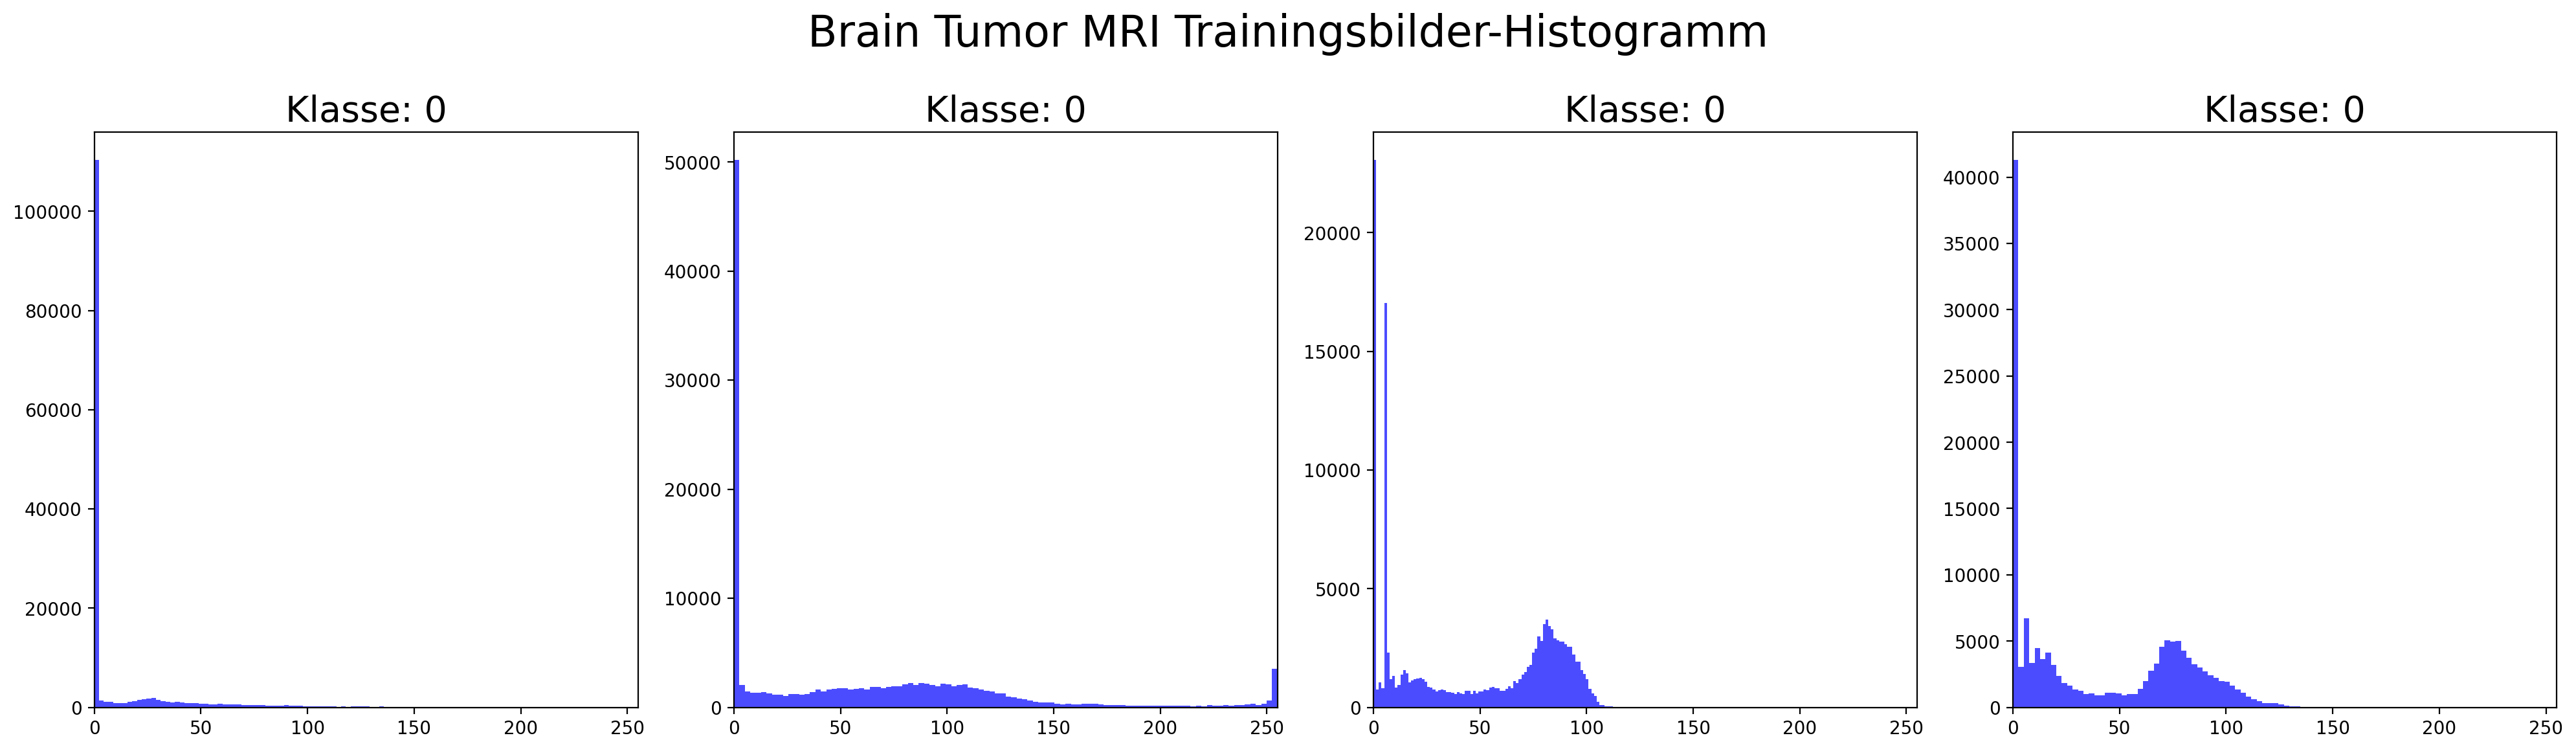
\includegraphics[width=\linewidth]{01-images/03-data/brain-klasse0-hist.png}
    \caption{Histogramm der Pixelverteilung von Abbildung \ref{fig:brain-beispiele-klasse0}}
    \label{fig:brain-klasse0-hist}
\end{figure}

\begin{figure}[H]
    \centering
    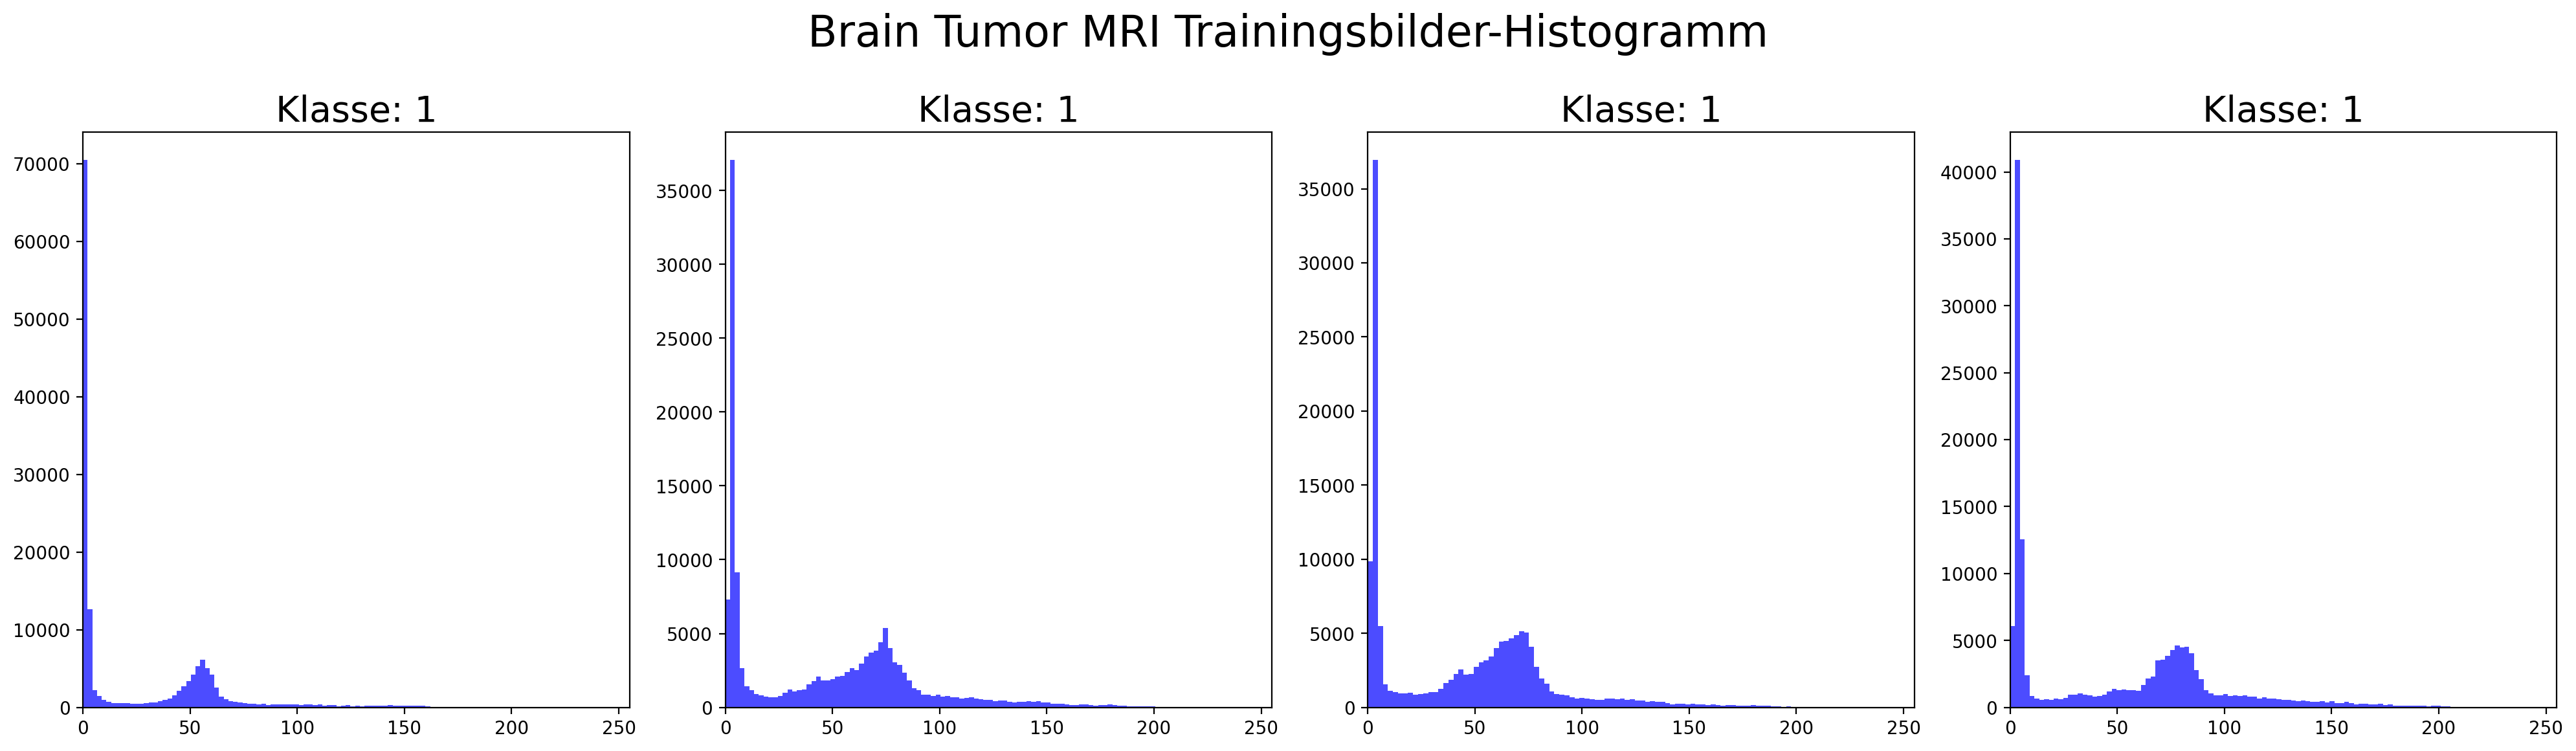
\includegraphics[width=\linewidth]{01-images/03-data/brain-klasse1-hist.png}
    \caption{Histogramm der Pixelverteilung von Abbildung \ref{fig:brain-beispiele-klasse1}}
    \label{fig:brain-klasse1-hist}
\end{figure}

Niedrige Pixelwerte in einem Bild weisen darauf hin, dass viele dunkle Bereiche vorhanden sind. Dies deutet darauf hin, dass es sich um den Hintergrund der MRI-Bilder handelt, der einen Grossteil der Informationen ausmacht, jedoch keine relevanten Details enthält.

\subsubsection{Datenverteilung} \label{chap:brain-datenverteilung}
Wie in Kapitel \ref{chap:COVID19-datenverteilung} beschrieben, stellte sich auch beim MRI-Datensatz das Problem der Performance auf den Testmetriken.

\paragraph{Pixelverteilung} \label{chap:brain-pixelverteilung}
Das Vorgehen, das in Kapitel \ref{chap:COVID19-pixelverteilung} beschrieben wird, nutzen wir ebenfalls für die Partitionierung des Hirntumor Datensatzes. Abbildung \ref{fig:brain-datapartition-pixelverteilung-histo} zeigt die Histogramme der Pixelwerte für jede Datenpartition.

\begin{figure}[H]
    \centering
    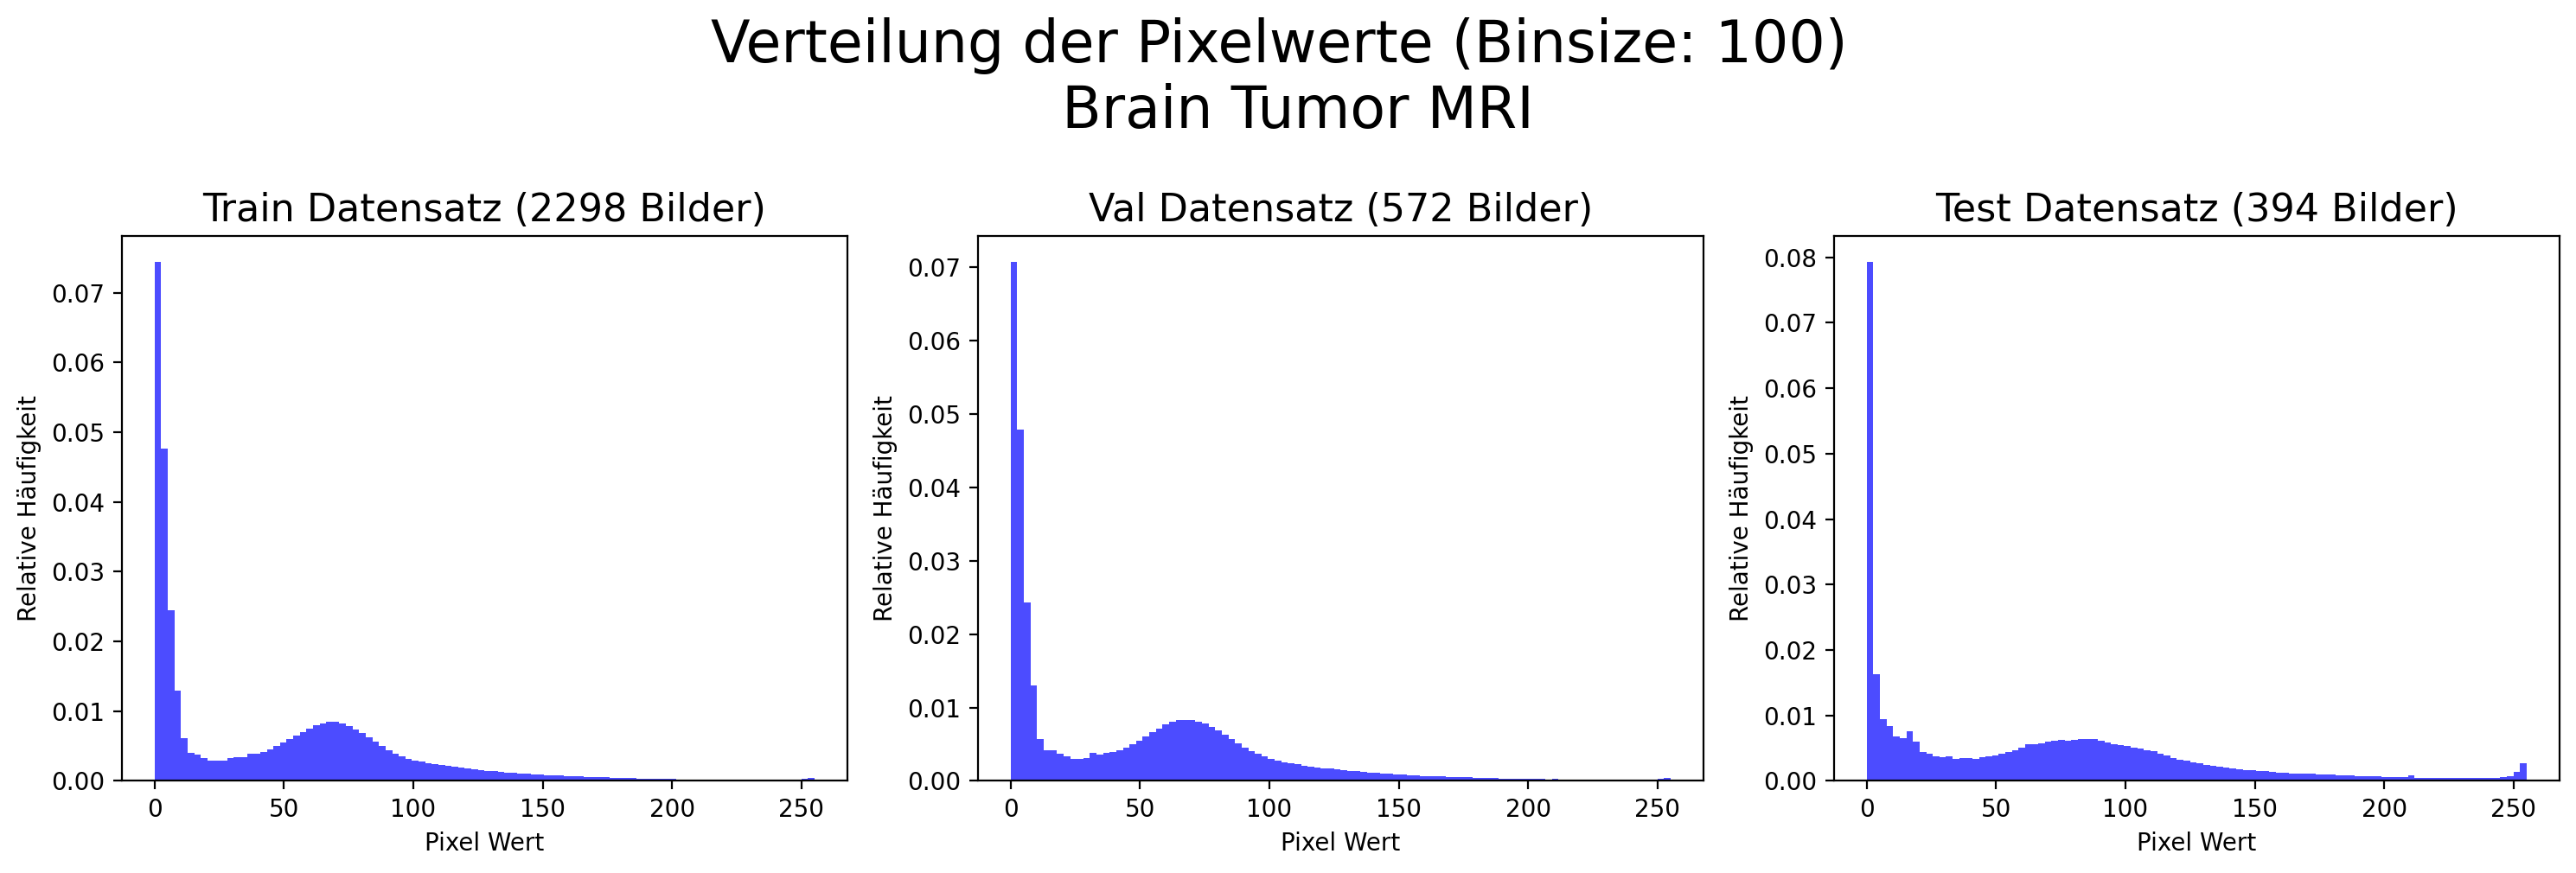
\includegraphics[width=\linewidth]{01-images/03-data/brain-Pixelverteilung-Partitionen.png}
    \caption{Histogramme der Pixelverteilung von Hirntumor in jeder Datenpartition}
    \label{fig:brain-datapartition-pixelverteilung-histo}
\end{figure}

Ein ähnliches Muster wie in Abbildung \ref{fig:covid-datapartition-pixelverteilung-histo}, das durch einen deutlichen Buckel gekennzeichnet ist, zeigt sich auch in diesem Hirntumor-Datensatz, jedoch mit einer Peakverschiebung. In den Hirntumor Histogrammen tritt dieser Peak typischerweise bei einem Pixelwert von etwa 80 auf. Sowohl die Trainings- als auch die Validierungspartition weisen ein vergleichbares Muster auf. In der Testpartition ist der Buckel allerdings weniger stark ausgeprägt. Zudem kommt es ab einem Pixelwert von 250 zu einem markanten Anstieg, der am Ende des Histogramms einen Ausschlag verursacht. Eine mögliche Erklärung hierfür ist, dass die Testdatenpartition aus einer anderen Verteilung stammt.

\paragraph{Pixelmittelwerte} \label{chap:Differenzenbilder-TestProblemEda2-mri}
Auch bei den Pixelmittelwerten erfolgt das Vorgehen analog zu dem in Kapitel \ref{chap:COVID19-pixelmittelwert} beschriebenen Verfahren.

\begin{figure}[H]
    \centering
    \begin{subfigure}[b]{0.49\linewidth}
        \centering
        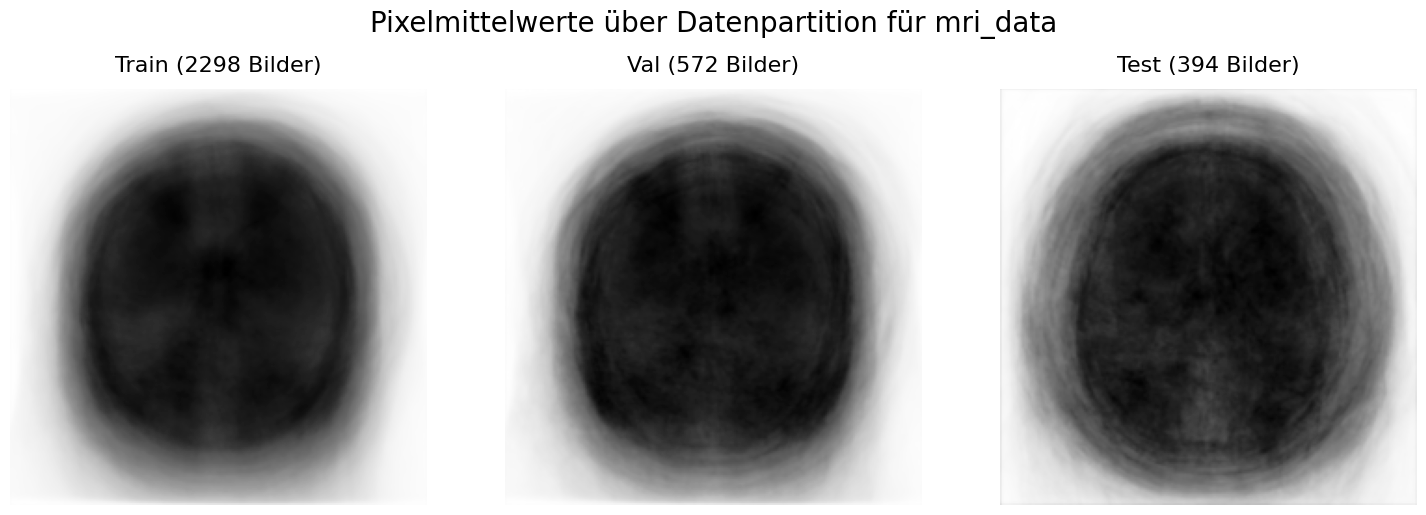
\includegraphics[width=\linewidth]{01-images/03-data/brain-pixelmittelwerte.png}
        \caption{Visuelle Darstellung der Pixelmittelwerte von aller Hirntumor pro Datenpartition}
        \label{fig:brain-pixelmittelwert-full}
    \end{subfigure}
    \hfill
    \begin{subfigure}[b]{0.49\linewidth}
        \centering
        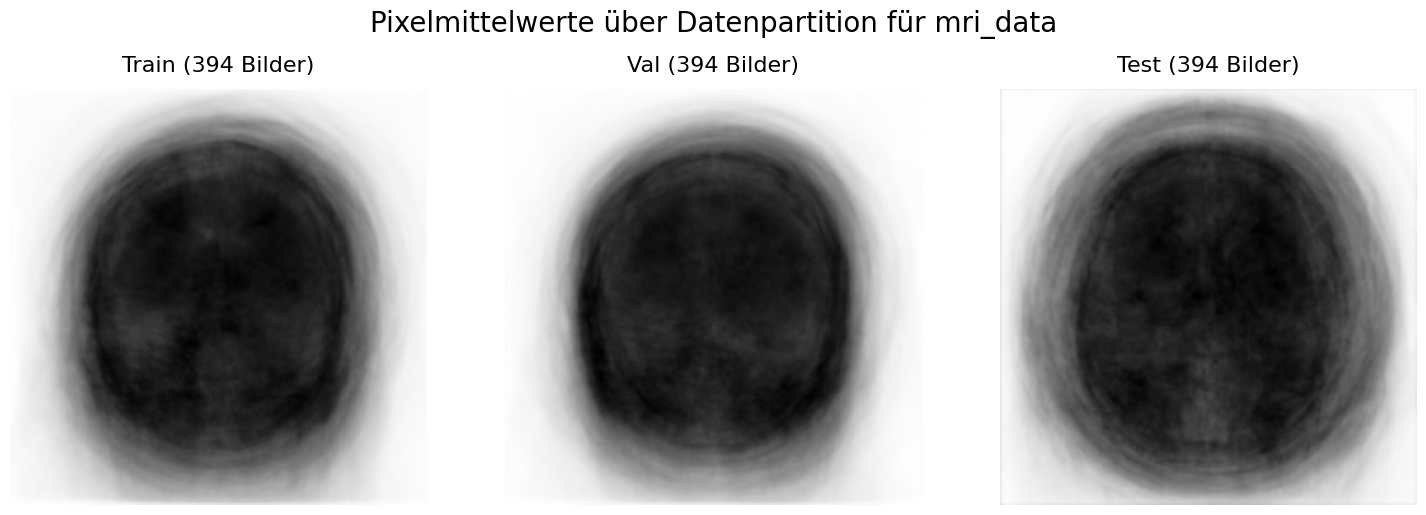
\includegraphics[width=\linewidth]{01-images/03-data/brain-pixelmittelwert-subsample-train.png}
        \caption{Visuelle Darstellung der Pixelmittelwerte einer Teilmenge von Hirntumor Bildern Datenpartition}
        \label{fig:brain-pixelmittelwert-subsample}
    \end{subfigure}
    \caption{Vergleich der Pixelmittelwerte von Hirntumor Bildern}
    \label{fig:brain-pixelmittelwert-comparison}
\end{figure}

Abbildung \ref{fig:brain-pixelmittelwert-full} zeigt die Differenzbilder der Pixelmittelwerte für alle Partitionen der Hirntumordaten. In allen drei Partitionen ist ein dunkler Kreis erkennbar. Feine Strukturen des Gehirns sind sowohl in der Validierungs- als auch in der Testpartition sichtbar, wobei diese Strukturen in der Testpartition deutlicher hervortreten als in der Validierungspartition. Zudem ist in der Testpartition erkennbar, dass die Pixelwerte ausserhalb des Kreises durchschnittlich höher und häufiger sind als in den Trainings- und Validierungspartitionen. Weiterhin zeigt sich ein Rand bei der Testpartition, was darauf hindeutet, dass die Testdaten möglicherweise eine höhere Variabilität oder eine andere Verteilung aufweisen als die Trainings- und Validierungsdaten. Die Visualisierung der Pixelmittelwerte mittels einer Teilmenge der Hirntumorbilder zeigt ebenfalls, dass die Anzahl der Bilder die Visualisierung visuell nicht gross verändert.

\paragraph{Differenzbilder} \label{chap:brain-differenzenbilder}
Für die Differenzbilder der Hirntumor Daten, wurde analog wie im Kapitel \ref{chap:COVID19-differenzbilder} die Heatmap Abbildung \ref{chap:brain-differenzenbilder} erstellt. Als Grundlagen zur Berechnung der Differenzen dienen die Pixelmittelwerte aus Abbildung \ref{fig:brain-pixelmittelwert-full}.

\begin{figure}[H]
    \centering
    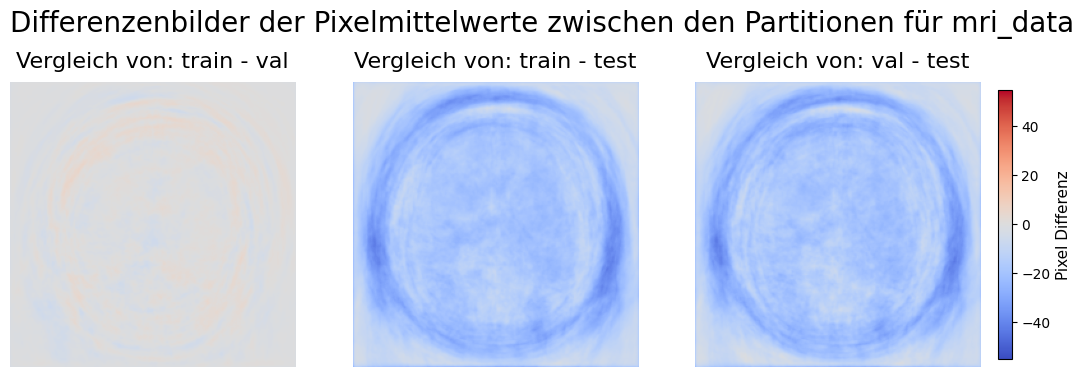
\includegraphics[width=\linewidth]{01-images/03-data/brain-differenzenbilder.png}
    \caption{Differenzbilder von Hirntumor in jeder Datenpartition}
    \label{fig:chap:brain-differenzenbilder}
\end{figure}

Dieser Plot zeigt Differenzbilder der Pixelmittelwerte zwischen verschiedenen Datenpartitionen für Hirntumoren. Drei Heatmap-Visualisierungen stellen die Differenzen zwischen den folgenden Partitionen dar.

Der Plot links zeigt die Differenz zwischen Trainings- und Validierungspartition. Die Berechnung erfolgt durch Subtraktion der Validierungsdaten von den Trainingsdaten. Hier wird erkennbar, dass die Differenz relativ klein ist im Vergleich zu den anderen Visualisierungen.

Die Plots in der Mitte und rechts zeigen die Differenzen zwischen den Trainings-, Validierungs- und Testdaten. Diese Differenzen wurden durch die Subtraktion der Testdaten von den Validierungs- und Trainingsdaten berechnet. Die Plots verdeutlichen, dass die Testdaten eine starke Abweichung aufweisen. Sowohl die Trainings- als auch die Validierungsdaten haben im Durchschnitt höhere Werte als die Testdaten, was zu negativen Differenzwerten führt und somit ein blaues Muster in den Plots erzeugt. Auffällig ist dabei insbesondere ein blaues Ringmuster.

\newpage